\documentclass[12pt]{article}
\usepackage{amssymb,mathtools}
\usepackage[margin=1in]{geometry}
\usepackage{fancyhdr}
\usepackage{circuitikz}
\usepackage{graphicx}
\graphicspath{ {./Figures/} }
\usepackage{amsmath}
\usepackage{ragged2e}
\usepackage{subcaption} 
\usepackage{float}
\usepackage{cancel}
\usepackage{siunitx}
\pagestyle{fancy}
\usepackage[shortlabels]{enumitem}
\usepackage{mathtools}
\newcommand*{\permcomb}[4][0mu]{{{}^{#3}\mkern#1#2_{#4}}}
\newcommand*{\Comb}[2]{{}^{#1}C_{#2}}%
\DeclarePairedDelimiter\ceil{\lceil}{\rceil}
\DeclarePairedDelimiter\floor{\lfloor}{\rfloor}
\setlength{\headheight}{15 pt}
\lhead{Georgy Antonov}
\chead{HW 3}
\rhead{Neural Dynamics}

\begin{document}\noindent


\noindent\textbf{Question 1. Simulation of a multi-compartment model of a passive neurite.}
\begin{enumerate}
        \begin{figure}[h]
            \centering
            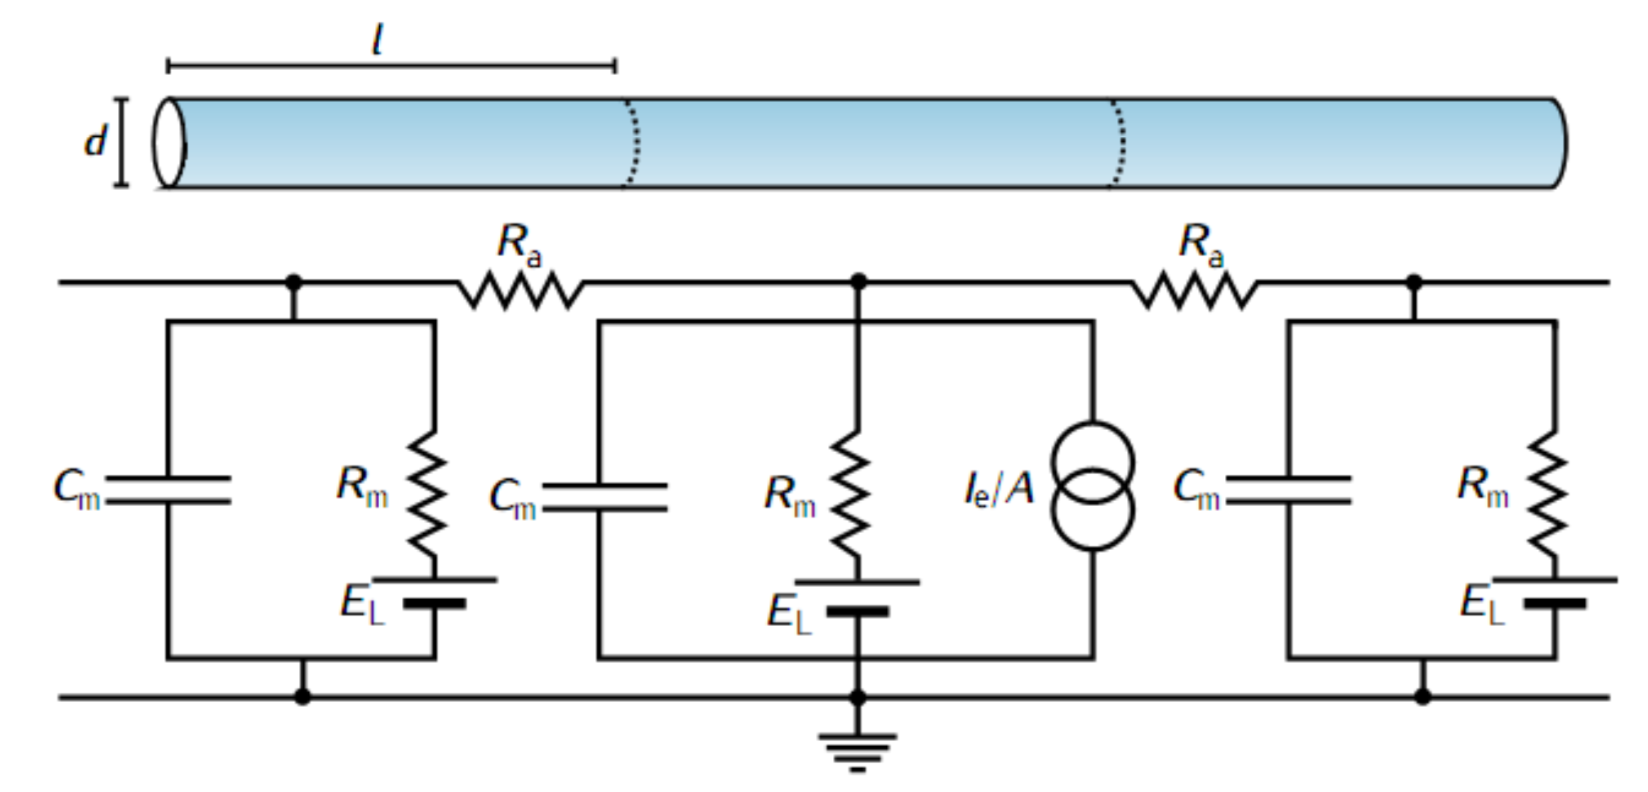
\includegraphics[width=0.7\textwidth]{model.png}
            \caption{Multi-compartment model.}
        \end{figure}
    \item[1.1] In the previous homework we solved for the voltage responses of a two-compartment model. Recall that
    \begin{align*}
        C_{m}\frac{dV_{1}(t)}{dt} &= \frac{E_{m} - V_{1}(t)}{R_m} + \frac{V_{2}(t) - V_{1}(t)}{R_{a}} + I_{e}(t)\\
        C_{m}\frac{dV_{2}(t)}{dt} &= \frac{V_{1}(t) - V_{2}(t)}{R_{a}} + \frac{E_{m} - V_{2}(t)}{R_m}
    \end{align*}
    We need to generalise this to an n-compartment model where $n \geqslant 2$ and arbitrary current $I_{e}(t)$ can be injected into 
    any of the n compartments.\\
    \\
    Following the diagram in Figure 1, we observe that
    $$I_{e, 2}(t) = C_{m}\frac{dV_{2}(t)}{dt} + \frac{V_{2}(t) - E_{L}}{R_{m}} + \frac{V_{2}(t) - V_{3}(t)}{R_{a}} + \frac{V_{2}(t) - V_{1}(t)}{R_{a}}$$
    Where the compartments are labelled 1-3 starting from the right hand side.\\
    \\
    Rearranging yeilds
    $$C_{m}\frac{dV_{2}(t)}{dt} = \frac{E_{L} - V_{2}(t)}{R_{m}} + \frac{V_{3}(t) - V_{2}(t)}{R_{a}} + \frac{V_{1}(t) - V_{2}(t)}{R_{a}} + I_{e, 2}(t)$$
    Note that we have the middle compartment 2 expressed in terms of its neighbouring compartments 1 \& 3. This can thus be generalised as
    \begin{equation} \label{eq1}
        \frac{dV_{j}(t)}{dt} = \frac{E_{L} - V_{j}(t)}{\tau_{m}} + \frac{1}{C_{m}}\left(\frac{V_{j+1}(t) - V_{j}(t)}{R_{a}} + \frac{V_{j-1}(t) - V_{j}(t)}{R_{a}}\right) + \frac{1}{C_{m}}I_{e, j}(t)
    \end{equation}
    Equation \ref{eq1} is known as the fundamental equation of a compartmental model. For the compartments without any current injected the response will look 
    the same as in equation \ref{eq1} but lacking the current term and dependent on the direction of the current flow. 
    Thus, if we use the same numbering scheme, then for compartment i where $0 < i < j$, we have
    $$\frac{dV_{i}(t)}{dt} = \frac{E_{L} - V_{i}(t)}{\tau_{m}} + \frac{1}{C_{m}}\left(\frac{V_{i-1}(t) - 2V_{i}(t) + V_{i+1}(t)}{R_{a}}\right)$$
    Similarly, for compartment i where $j < i < N$ where $N$ is the number of compartments, we have
    $$\frac{dV_{i}(t)}{dt} = \frac{E_{L} - V_{i}(t)}{\tau_{m}} + \frac{1}{C_{m}}\left(\frac{V_{i+1}(t) - 2V_{i}(t) + V_{i-1}(t)}{R_{a}}\right)$$
    \textit{Nota bene} for the terminal compartments (i.e. when $i=0$ or $i=N$ we have to make use of the boundary conditions as 
    shown in Figure 2.
    \begin{figure}[h]
        \centering
        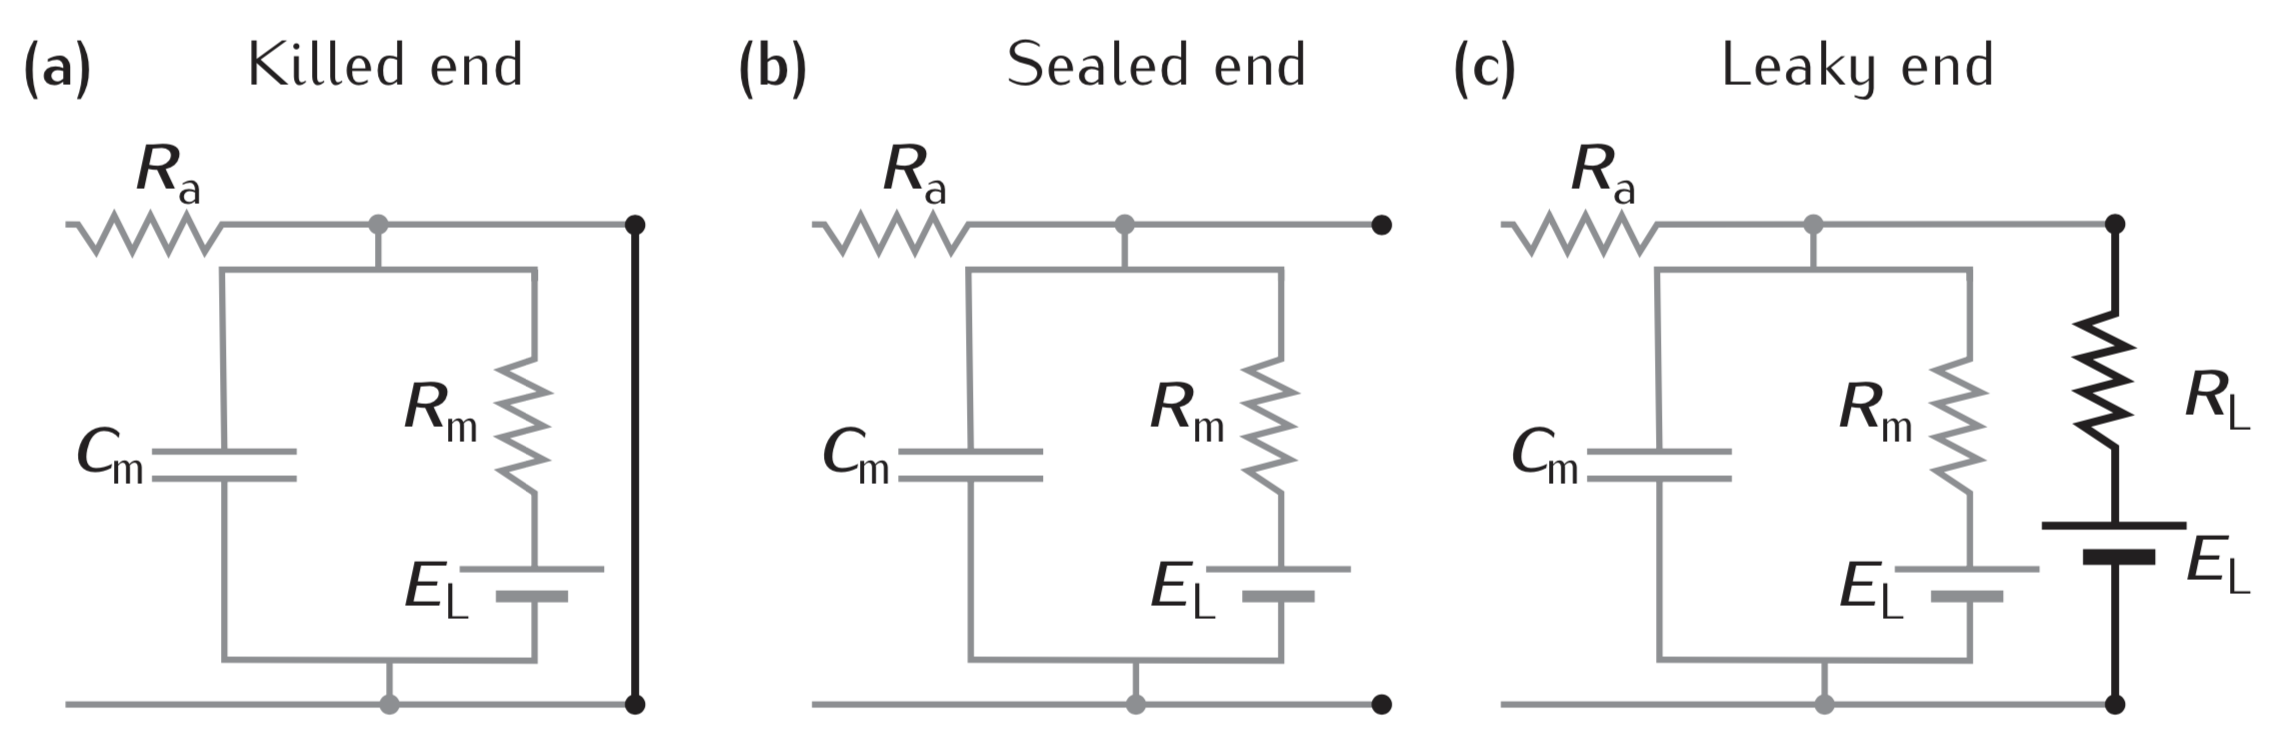
\includegraphics[width=0.9\textwidth]{boundary.png}
        \caption{Boundary conditions for the terminal compartments.}
    \end{figure}
    For the killed end (Dirichlet) boundary condition the neurite's intracellular environment is in contact with the extracellular medium, 
    and hence the potential $V_{i}$ for that compartment is set to 0. For the sealed end (Neumann) boundary condition, we assume that the resistance 
    is so high that no current can pass through the end. Since the axial current is proportional to the gradient of the membrane potential, no current 
    implies zero potential gradient.
    \item[1.2] Equation \ref{eq1} can be approximated with the forward Euler method as shown below
    \begin{align*}
        \frac{V_{j}(t + \Delta t) - V_{j}(t)}{\Delta t} &= \frac{E_{L} - V_{j}(t)}{\tau_{m}} + \frac{1}{C_{m}}\left(\frac{V_{j+1}(t) - V_{j}(t)}{R_{a}} + \frac{V_{j-1}(t) - V_{j}(t)}{R_{a}}\right) + \frac{1}{C_{m}}I_{e, j}(t)
    \end{align*}
    \begin{align*}
        \implies V_{j}(t + \Delta t) = V_{j}(t) &+ \Delta t \left( \frac{E_{L} - V_{j}(t)}{\tau_{m}} + \frac{1}{C_{m}} \left( \frac{V_{j+1}(t) - V_{j}(t)}{R_{a}} + \frac{V_{j-1}(t) - V_{j}(t)}{R_{a}}\right) \right)\\
        &+ \frac{\Delta t}{C_{m}}I_{e, j}(t)
    \end{align*}
    Now, we simulate this with step current given below 
    \[
    I_{e}(j, t)= 
    \begin{cases}
        0, & (t < t_{e}) \vee (j \neq j_{e})\\
        10 \, \text{pA} ,              & (t_{e} \leqslant t) \wedge (j = j_{e})\\
    \end{cases}
    \]
    We assume $N = 50$ compartments where the first compartment is terminated as a 'sealed end' 
    and the last compartment is terminated as a 'killed end'. We also assume the following electrical properties
    \begin{enumerate}
        \item[a)] Membrane capacitance $C_{m} = 62.8 \, \text{pF}$
        \item[b)] Membrane resistance $R_{m} = 1.59 \, \text{G\si{\ohm}}$
        \item[c)] Axial resistance $R_{a} = 0.0318 \, \text{G\si{\ohm}}$
        \item[d)] $E_{L} = E_{m} = 0 \, \text{V}$
    \end{enumerate}
\end{enumerate}
\end{document}
